\documentclass[0-protokol.tex]{subfiles}
\begin{document}
Termistor je polovodičová součástka, jejíž odpor závisí na teplotě, nejčastěji s teplotou klesá. To je způsobeno zvýšením koncentrace nositelů náboje či zvýšení jejich pohyblivosti při rostoucí teplotě. V obou případech Závisí odpor termistoru $R_t$ na teplotě $T$ vztahem 
\begin{equation} \label{eq:odpor_teplota}
R_t = R_\infty \exp(\frac{B}{T}).
\end{equation}
Konstanta $R_\infty$ závisí na materiálu a rozměrech termistoru, veličina charakterizuje v prvním případě teplotní citlivost součástky, v případě druhém změnu pohyblivosti nositelů náboje.

Klesající odpor s rostoucí teplotou znamená, že termistor má záporný teplotní součinitel odporu $\alpha$. Ten navíc není konstantní, ale závislý na teplotě podle
\begin{equation} \label{eq:alpha}
\alpha = -\frac{B}{T^2}.
\end{equation}

Aktivační energie je energie potřebná k ionizaci příměsi, tedy k tomu, aby se elektron dostal z příměsového atomu do vodivostního pásu. V literatuře se zpravidla uvádí v jednotkách $\si{\electronvolt}$ nebo $\si{\joule\per\mole}$. Lze vypočítat jako 
\begin{equation} \label{eq:delta_U}
\Delta U = 2RB,
\end{equation}
kde $R = \SI{8.314}{\joule\per\mole\per\kelvin}$ je plynová konstanta.

Konstanty $B$ a $R_\infty$ nejlépe získáme z lineární regrese grafu rovnice 
\begin{equation} \label{eq:log_R}
\log R = \log R_\infty + \frac{B}{T}.
\end{equation}

Pomocí zapojení \ref{fig:staticka_charakteristika} naměříme statickou voltampérovou charakteristiku termistoru. Teplotu v bodě maxima spočítáme podle vzorce 
\begin{equation} \label{eq:teplota_v_max}
T_m = \frac{1}{2} (B - \sqrt{B(B-4T_0)}),
\end{equation}
kde $T_0$ je teplota okolí. Pomocí této hodnoty pak stanovíme tepelný odpor $K$ pomocí 
\begin{equation} \label{eq:K}   
K = \frac{T_m-T_0}{U_m I_m}.
\end{equation}  
Indexem $m$ jsou označeny hodnoty při maximálním napětí na termistoru.

\begin{figure}[H]
\centering
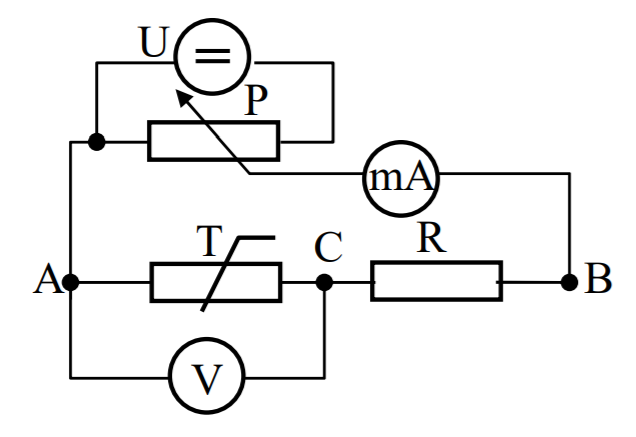
\includegraphics[scale=0.5]{staticka_charakteristika}
\caption{Zapojení pro měření statické charakteristiky termistoru}
\label{fig:staticka_charakteristika}
\end{figure}

Pomocí schématu \ref{fig:zavislost_na_teplote} měříme závislost odporu termistoru na teplotě. Teplotu měříme platinovým odporovým teploměrem, hodnoty teplot v kelvinech získáme z naměřených odporů $R_{Pt}$ pomocí vztahu
\begin{equation} \label{eq:teplota_z_odporu}
T = \frac{R_{Pt} - R_0}{\alpha_{Pt}R_0} + \num{273.15},
\end{equation}
přičemž $R_0 = \SI{100}{\ohm}$ je odpor teploměru při teplotě $\SI{273.15}{\kelvin}$ a $\alpha_{Pt} = \SI{3.85e-3}{\per\kelvin}$ je teplotní součinitel odporu teploměru.

\begin{figure}[H]
\centering
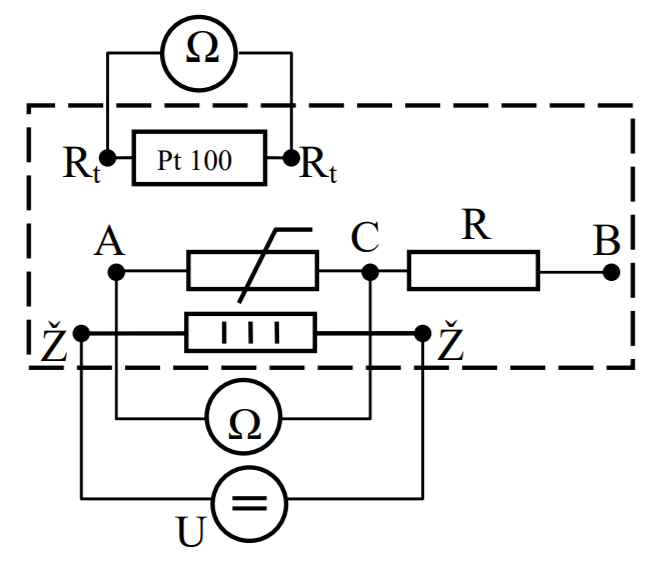
\includegraphics[scale=0.5]{zavislost_na_teplote}
\caption{Schéma pro měření závislosti odporu termistoru na teplotě}
\label{fig:zavislost_na_teplote}
\end{figure}

\end{document}
